\documentclass{uoc-es}[2008/10/15 v2.1 UOC document class]%Versi\'on 2.1 de la clase UOC

% Crec que les tres instruccions seguents no son necessaries perque ja ho inclou el paquet uoc-es?
%\usepackage[latin1]{inputenc} % Juego de codigos ampliado en windows
%\usepackage[utf8]{inputenc} % Juego de codigos ampliado en linux
%\usepackage[spanish]{babel} % Juego de codigos ampliado en windowsLenguaje español

\usepackage{estiluoc} % Estilo UOC

%\usepyackage{mathstone} %Tipograf\'ia Stone
%\usepackage{dcolumn} %Definici\'on de columnas de tablas con decimales
%\newcolumntype{d}{D{,}{,}{2}}

\definecolor{miorange}{rgb}{0.91, 0.43, 0.0}

%%%%%%%%%%%%%% Portada del m\'odulo %%%%%%%%%%%%%%%%%%%%%%%%%%%%%%%%%%%%%%%%


\title{An\'alisis de datos de microarrays} %T\'itulo del m\'odul

%\renewcommand{\subtitle}{Exploraci\'on y Control de Calidad} %Subt\'itulo del m\'odulo

\author{Alex S\'anchez-Pla y M. Carme Ru\'iz de Villa\\
Departament d'Estad\'istica. Universitat de Barcelona.\\
Facultat de Biologia. Avda. Diagonal 643. 08028 Barcelona. Spain.\\
\texttt{asanchez@ub.edu;mruiz\_de\_villa@ub.edu}}

\newcommand{\modul}{M\'odulo 6} %N\'umero de m\'odulo en la portada
\newcommand{\credits}{xx} %Cr\'editos
\renewcommand{\nroregistre}{PID_00191030} %Codigo de m\'odulo

%\newcommand{\R}{\textbf{R}}

%%%%%%%%%%%%%% Encabezado de p\'aginas %%%%%%%%%%%%%%%%%%%%%%%%%%%%%%%%%%%%%%


\newcommand{\nommodul}{An\'alisis de datos de microarrays} %Codigo del m\'odulo en encabezado.
\newcommand{\modulEncap}{$\text{ }\bullet$ M\'odulo XXX} %M\'odulo en encabezado.

%%%%%%%%%%%%%% Espacio para definir nuevas instrucciones  %%%%%%%%%%%%%%%%%%%%

% ESCRIBID AQUÍ LAS NUEVAS INSTRUCCIONES

\usepackage{hyperref} % Estilo UOC
\usepackage{Sweave}
\usepackage{supertabular}
\usepackage{underscore}

\newcommand{\Rfunction}[1]{{\texttt{#1}}}
\newcommand{\Rmethod}[1]{{\texttt{#1}}}

\newcommand{\Robject}[1]{{\texttt{#1}}}
\newcommand{\Rpackage}[1]{{\textit{#1}}}
\newcommand{\Rclass}[1]{{\textit{#1}}}

\newcommand{\bit}{\begin{itemize}}
\newcommand{\eit}{\end{itemize}}
\newcommand{\ben}{\begin{enumerate}}
\newcommand{\een}{\end{enumerate}}

\newcounter{MiEnum}
%%%%%%%%%%%%%% Inicio del m\'odulo %%%%%%%%%%%%%%%%%%%%%%%%%%%%%%%%%%%%%%%%%%%%

\includeonly{capitulo4,capituloFinal}

\begin{document}


\maketitle

%%%%%%%%%%%%% Pàgina blanca darrera la portada
\newpage
\mbox{ }
\thispagestyle{empty}
\newpage
%%%%%%%%%%%%%%%%%%%%%%%%%%%%%%%%%%%%%%%

\tableofcontents

%%%%%%%%%%%%%%%%%%%%%%%%%%%%%%%%%%%%%%%

\setcounter{modul}{1}
\normalbaroutside % Paquet ``programa.sty''
\frenchspacing

%%%%%%%%%%%%%%%%%%%%%%%%%%%
\part{Preliminares}

\include{capitulo0}
\include{capitulo1}
\include{capitulo2}
\include{capitulo3}
\include{casoResuelto1}


\part{An\'alisis de datos de microarrays}

\chapter{El proceso de an\'alisis de datos de microarray (MDA)\label{MDAProcess}}

\section{Introducci\'on}

Este cap\'itulo es una corta transici\'on entre la primera parte del curso, en la que se han presentado los conceptos y herramientas b\'asicos y la segunda en donde se presentan por separado y con mayor detalle los m\'etodos de an\'alisis de datos de microarrays.

Su objetivo por tanto es ofrecer una visi\'on \emph{de conjunto} que sirva de gu\'ia (``roadmap'') para los cap\'itulos siguientes de forma que sin perder el detalle de cada uno de ellos tengamos conciencia de en que punto del proceso general nos encontramos.

El cap\'itulo se estructura en dos partes. En la primera se presentan brevemente algunos de los problemas que t\'ipicamente se puede querer estudiar con microarrays u otras t\'ecnicas similares de an\'alisis de datos de alto rendimiento. A continuaci\'on se presenta lo que se ha llamdo aqu\'i el \emph{proceso de an\'alisis de microarrays}. Finalmente se intoducen algunos casos reales que, a modo de ejemplo se utilizar\'an en los cap\'itulos siguientes.

\section{Tipos de estudios}

Los microarrays y otras tecnolog\'ias de alto rendimiento se han aplicado a multitud de investigaciones, de tipus muy diversos que van desde estudio del cancer  (\cite{alizadeh:2000, Golub:1999, vantveer:2002}) al de la germinaci\'on y la maduraci\'on del tomate (\cite{Moore:2002}). A pesar de ello no resulta complicado clasificar los estudios realizados en algunos de los grandes bloques que se describen a continuaci\'on. La clasificaci\'on est\'a basada en el excelente texto de Simon y colegas (\cite{Simon:2003}) y aunque se origina en problemas de microarrays se puede aplicar f\'acilmente a estudios de gen\'omica o ultrasecuenciaci\'on.

\subsection{Comparaci\'on de grupos o \emph{Class comparison}}

El objetivo de los estudios comparativos es determinar si los perfiles de expresi\'on g\'enica difieren entre grupos previamente identificados. Tambi\'en se conoce estos estudios como de \emph{selecci\'on de  genes diferencialmente expresados} y son, sin duda los m\'as habituales. Los grupos pueden representar una gran variedad de condiciones, desde distintos tejidos a distintos tratamientos o m\'ultiples combinaciones de factores experimentales.

El an\'alisis de este tipo de experimentos, que se describe en el cap\'itulo sobre selecci\'on de genes diferencialmente expresados utiliza herramientas estad\'isticas como las pruebas de comparaci\'on de grupos param\'etricas (t de Student) o no (test de Mann-Whitney) o diversos m\'etodos de an\'alisis de la varianza.

Entre los ejemplos de la secci\'on ~\ref{c4examples} los casos  ~\ref{celltypes}, ~\ref{estrogen} o ~\ref{CCL4} hacen referencia a estudios comparativos.

\subsection{Predicci\'on de clase o \emph{Class prediction}}

La predicci\'on de clase puede confundirse con la selecci\'on de genes en tanto que disponemos de clases predefinidas pero su objetivo es distinto, ya que no pretende simplemente buscar genes cuya expresi\'on sea distinta entre dichos grupos sino genes que puedan ser utilizados para identificar a que clase pertenece un ``nuevo'' individuo dado cuya clase es ``a priori'' desconocida. El proceso de predicci\'on suele empezar con una selecci\'on de genes informativos, que pueden ser, o no, los mismos que se obtendr\'ian si aplic\'aramos los m\'etodos del apartado anterior, seguida de la construcci\'on de un modelo de predicci\'on y, lo que es m\'as importante, de la verificaci\'on o validaci\'on de dicho modelo con unos datos nuevos independientes de los utilizados para el desarrollo del modelo.

Aunque el inter\'es de la predicci\'on de clase es muy alto se trata de un procedimiento mucho m\'as complejo y con m\'as posibilidades de error que la simple selecci\'on de genes diferencialmente expresados.

Entre los ejemplos de la secci\'on ~\ref{c4examples} el caso  ~\ref{golub} trata de un problema de predicci\'on, a la vez que uno de descubrimiento de clases.

\subsection{Descubrimiento de clases o \emph{Class discovery}}

Un problema distinto a los descritos se presenta cuando no se conoce las clases en que se agrupan los individuos. En este caso de lo que se trata es de encontrar grupos entre los datos que permitan reunir a los individuos m\'as parecidos entre si y distintos de los de los dem\'as grupos. Los m\'etodos estad\'isticos que se emplearan en estos casos se conocen como \emph{an\'alisis de clusters} y no son tan complejos como los de predicci\'on de clase aunque algunos aspectos como por ejemplo la definici\'on del n\'umero de grupos no resulta tampoco sencillo.

Entre los ejemplos de la secci\'on \ref{c4examples} tanto el caso \texttt{golub}, en parte, como el ~\ref{breastTum}  tratan problemas de descubrimiento de clases.

Una curiosidad del campo de la estad\'istica es que el t\'ermino clasificaci\'on aparece usado de forma indistinta para referirse a problemas de predicic\'on de clase o de descubrimiento de clase.

\subsection{Otros tipos de estudios}

Una vez identificados los principales tipos de estudios quedan muchos que no coinciden plenamente con ninguno de ellos. Sin entrar en detalles podemos se\~nalar los estudios de evoluci\'on a lo largo del tiempo  (``time course''), los de significaci\'on biol\'ogica (``Gene Enrichment Analysis'', ``Gene Set Enrichment Analysis'', ...) , los que buscan relaciones entre los genes (``network analysis'' o ``pathway analysis''). De momento con conocer e identificar los tres grandes bloques mencionados resultar\'a m\'as que suficiente.


\section{Algunos ejemplos concretos \label{c4examples}}

Una de las dificultades con que se encuentra la persona que comienza en el an\'alisis de datos de microarrays es de donde obtener ejemplos concretos con los que pr\'acticar las t\'ecnicas que est\'a aprendiendo.

No es dif\'icil encontrar datos de microarrays en internet por lo que
se han seleccionado algunos conjuntos de datos interesantes para
utilizarlos de ejemplo a lo largo del curso. Algunos de \'estos son
``populares'' en el sentido de que han sido utilizados en diversas
ocasiones y por lo tanto se encuentran bien documentados. Otros se han
escogido simplemente porque ilustran bien algunas de las ideas que se
desea exponer o por su accesibilidad.

Todos los datos corresponden a investigaciones publicadas por lo que no se describen exhaustivamente sin\'o que se expone brevemente el origen y objetivos del trabajo --incluyendo su clasificaci\'on seg\'un los grupos definidos en la secci\'on anterior-- y las caracter\'isticas perinentes para el an\'alisis como el tipo de microarrays, los grupos --si los hay-- o como acceder a los datos.

\subsection{Estudio de procesos regulados por citoquinas \label{celltypes}}
\underline{Efecto de la estimulaci\'on con LPS sobre los procesos regulados por citoquinas }

Este conjunto de datos, que se denominar\'a ``celltypes'', corresponde a un estudio realizado por Chelvarajan y sus colegas (\cite{Chelvarajan:2006}) que analizaron el efecto de la estimulaci\'on con lipopolisac\'aridos en la regulaci\'on por parte de citoquinas de ciertos procesos biol\'ogicos relacionados con la inflamaci\'on.

Este estudio es del tipo ``class comparison'' es decir su principal objetivo es la obtenci\'on de genes diferencialmente expresados entre dos o m\'as condiciones.

Los datos se encuentran disponibles en la base de datos p\'ublica \texttt{caarray} mantenida por el \emph{National Institute of Health (NIH)}, pero pueden descargarse de la p\'agina de materiales del curso para garantizar su disponibilidad.

\subsection{Clasificaci\'on molecular de la leucemia\label{golub}}

\underline{Clasificaci\'on molecular para distinguir variantes de leucemia mielobl\'astica aguda }

A finales de los a\~nos 90, Todd Golub y sus colaboradores (\cite{Golub:1999}) realizaron uno de los estudios m\'as populares hasta el momento con datos de microarrays. En \'el utilizaron microarrays de oligonucle\'otidos para 6817 genes humanos para mirar de encontrar una forma de distinguir (clasificar) tumores de pacientes con leucemia linfobl\'astica aguda (ALL) de aquellos que sufr\'ian de leucemia mieloide aguda (AML).
Adem\'as se interesaba por la posibilidad de descubrir subgrupos de forma que pudieran definirse variantes de cada una de estas patolog\'ias a nivel molecular.

La diversidad de objetivos del estudio lleva a clasificarlo tanto entre los del tipo de predicci\'on de clase como entre los que buscan descubrir nuievas clases o grupos en los datos.

Los datos de este estudio se encuentran disponibles en la web del instituto Broad, en donde se llev\'o a cabo (\href{http://www.broadinstitute.org}{http://www.broadinstitute.org}). Tambi\'en se encuentra disponible un paquete de \texttt{R} denominado \texttt{ALL} que permite utilizarlos directamente usando \texttt{R} y Bioconductor.

\subsection{Efecto del estrogeno y el tiempo de administraci\'on\label{estrogen}}

\underline{Efecto del tratamiento con estr\'ogenos en la expresi\'on de genes relacionados con c\'ancer de mama }

Scholtens y colegas (\cite{Scholtens:2004}) describen un estudio sobre el efecto de un tratamiento con estr\'ogenos y del tiempo transcurrido desde el tratamiento en la expresi\'on g\'enica en pacientes de c\'ancer de mama. Los investigadores supusieron que los genes asociados con una respuesta temprana podr\'ian considerarse dianas directas del tratamiento,
mientras que los que tardaron m\'as en hacerlo podr\'ian considerarse objetivos secundarios correspondientes a dianas m\'as alejadas en las
v\'ias metab\'olicas.

Estos datos han sido utilizados multitud de veces en los cursos de an\'alisis de microarrays realizados por el proyecto Bioconductor y se encuentran disponibles en forma de paquete de \texttt{R}, el paquete \texttt{estrogen}. Una cracater\'istica importante de este paquetes es el hecho de que en vez de los datos procesados proporciona  los datos ``crudos''en forma de archivos .CEL de Affymetrix. Esto permite una mayor flexibilidad a la hora de reutilizarlos lo que explica su popularidad.

\subsection{Efecto del CCL4 en la expresi\'on g\'enica\label{CCL4}}

\underline{Efecto del tratamiento con dimetilsulf\'oxido (DMSO) en la expresi\'on g\'enica }

Holger y colegas de la empresa LGC Ltd. en Teddington, Inglaterra realizaron unos expeimentos con microarrays de dos colores en los que trataron hepatocitos de rat\'on con tetraclorido de carbono (CCL4) o con dimetilsulf\'oxido (DMSO). El tetraclorido de carbono fue ampliamente utilizado en productos de limpieza o refrigeraci\'on para el hogar hasta que se detect\'o que pod\'ia tener efectos t\'oxicos e incluso cancer\'igenos. El DMSO es un solvente similar, sin efectos t\'oxicos conocidos, que se utiliz\'o como control negativo.

Los datos de este estudio no han sido publicados pero se encuentran disponibles en el paquete \texttt{CCL4} de bioconductor. Su inter\'es reside por un lado en que se trata de datos de microarrays de dos colores de la marca Agilent --en un momento en que la mayor\'ia de estudios se realizan con datos de un color. Aparte de esto cabe resaltar el hecho de que el paquete incluye, de forma similar al anterior, los datos ``crudos'' en forma de archivos de tipo ``Genepix'' uno de los programas populares para escanear im\'agenes generadas con microarrays de dos colores.

Este estudio es tambi\'en un estudio de comparaci\'on de clases cuyo objetivo principal es la selecci\'on de genes cuya expresi\'on se asocia al tratamiento con CCL4 o DMSO.


\subsection{An\'alisis de patrones en el ciclo celular\label{yeast}}

\underline{Busqueda de patrones de coexpresi\'on en datos de ciclo celular de levadura
}
Los datos de este ejemplo denominado \texttt{kidney} son datos ya normalizados referidos a la expresi\'on de los genes en distintos momentos del ciclo delular de la levadura e decir desde que concluye la divisi\'on celular hasta que se inicia la siguiente.

Los datos puede desargarse desde la p\'agina del proyecto ``Yeast Cell Cycle Project'' (Proyecto de estudio del ciclo celular de la levadura) en la direcci\'on:\\
\href{http://genome-www.stanford.edu/cellcycle/data/rawdata/}{http://genome-www.stanford.edu/cellcycle/data/rawdata/}.


\subsection{Recapitulaci\'on}

La tabla \ref{ejemplosEstudios} resume la lista de ejemplos que se utilizan en este manual indicando el nombre con que nos referiremos de aqu\'i en adelante a cada conjunto de datos as\' como algunas de sus carcater\'isticas.

\begin{table}[!h]
\titoltaula[0cm]{Tabla \ref{ejemplosEstudios}. Conjuntos de datos utilizados en este manual. Aparte del nombre (arbitrario y ``mnemot\'ecnico'') se indica el tipo de microarrays, el n\'umero de muestras, y el tipo de problema para el que se utilizaron originalmente.}
\begin{tabular}{|l|c|c|c|}
\hline
Nombre & Tipo & N. Muestras & Tipo de estudio  \\ \hline
\texttt{celltypes} & Un color (Affy, Mouse 4302) & 12 & Comparativo \\ \hline
\texttt{golub}     & Un color (Affy, HGU95A)  & 38  & Clasificaci\'on \\ \hline
\texttt{estrogen}  & Un color (Affy, HGU95A)  & 8 & Comparativo \\ \hline
\texttt{CCL4}     & Dos colores (Agilent, WG Rat Microarray)    & 16 & Comparativo \\ \hline
\texttt{breastTum} & Un color  (Affy, HGU95A) & 49 & Clasificaci\'on \\ \hline
\end{tabular}
\label{ejemplosEstudios}
\end{table}


\section{El proceso de an\'alisis de microarrays}

Una vez descritos los tipos de an\'alisis y algunos ejemplos podemos pasar a describir el proceso de an\'alisis de microarrays que se resume brevemente en la figura ~\ref{c04analysisProcess}.

El an\'alisis de microarrays, como la mayor\'ia de an\'alisis debe proceder de forma ordenada y siguiendo el m\'etodo cient\'ifico:
\begin{itemize}
\item La pregunta y su contexto nos servir\'an de gu\'ia para definir el \emph{Dise\~no experimental} adecuado.
\item El experimento se deber\'a realizar siguiendo las pautas decididas en el \emph{Dise\~no experimental} y los datos obtenidos
--que solemos denominar datos ``crudos'' o ``raw data''-- deber\'an someterse a los \emph{Controles de calidad adecuados} antes de continuar con su an\'alisis.
\item Una vez decidido si la calidad de los datos es aceptable pasaremos a prepararlos para el an\'alisis lo que puede incluir diversas formas
de \emph{preprocesado, o transformaciones} que a menudo se incluyen de forma general bajo el paraguas del t\'ermino \emph{normalizaci\'on}, aunque, como veremos se trata de conceptos distintos.
\item Los datos normalizados se utilizar\'an para los \emph{an\'alisis estad\'isticos} que hayamos decidido realizar durante el dise\~no experimental.
\item Finalmente los resultados de los an\'alisis ser\'an la base para una \emph{interpretaci\'on biol\'ogica} de los resultados del experimento.
\end{itemize}


\textD{Figura \ref{c04analysisProcess}}{El an\'alisis de microarrays puede ser f\'acilmente visualizado como un proceso que empieza por una
pregunta biol\'ogica y concluye con una interpretaci\'on de los resultados de los an\'alisis que, de alguna forma,
confiamos nos acerque un poco a la respuesta de la pregunta inicial.}

\vspace{-0.5cm}
\begin{figure}[!h]
\titolfigura[0cm]{Figura \ref{c04analysisProcess}. Proceso de an\'alisis de microarrays}
\label{c04analysisProcess}
\fbox{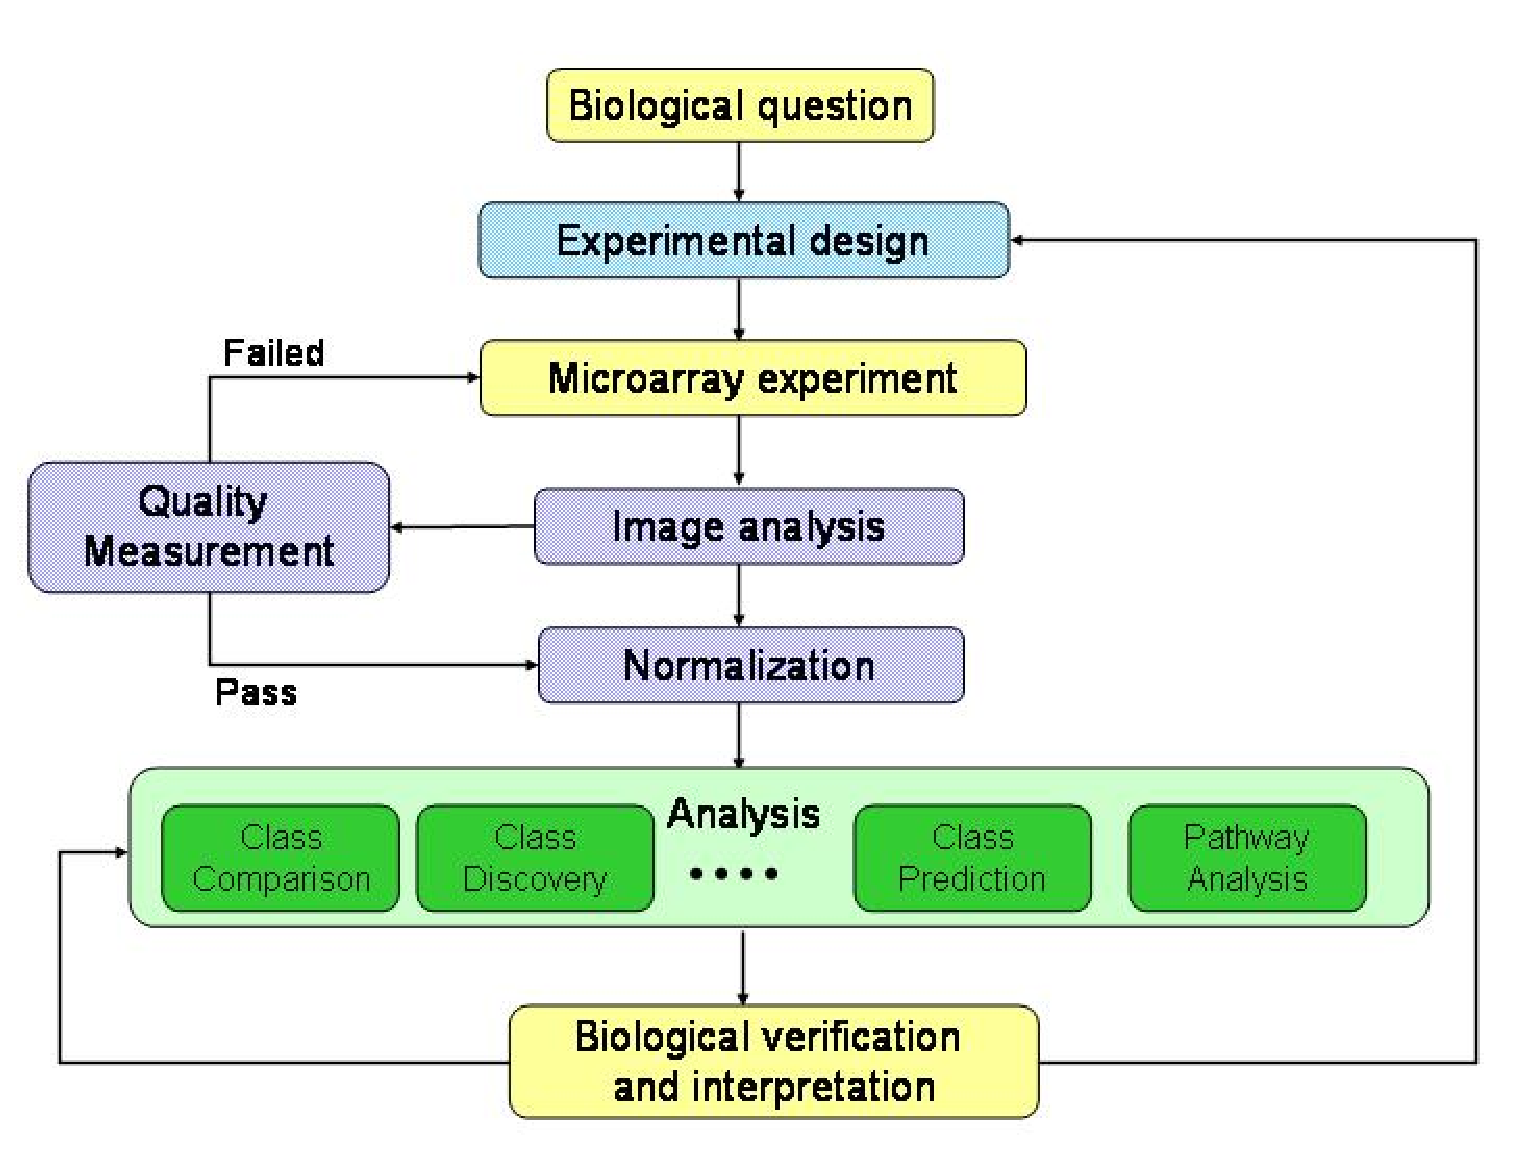
\includegraphics[height=6cm,width=0.75\textwidth]{epsimages/c04analysisProcess.eps}}
\end{figure}



El proceso descrito es b\'asicamente una forma razonable de proceder en general.
Los microarrays y otros datos gen\'omicos son diferentes en su naturaleza de
los datos cl\'asicos alrededor de los que se han desarrollado la mayor parte de
t\'ecnicas estad\'isticas. En consecuencia, en muchos casos ha sido necesario
adaptar las t\'ecnicas existentes o desarrollar otras nuevas para adecuarse a las nuevas situaciones encontradas.
Esto ha determinado que existan muchos m\'etodos para cada una de los pasos descritos anteriormente lo que da lugar a una grand\'isima cantidad de
posibilidades.

En la pr\'actica lo que suele hacerse es optar por utilizar algunos de los m\'etodos en los que hay un cierto consenso acerca de su calidad y
utilidad para cada problema. Allison (\cite{Allison:2006a}) repasa los puntos principales de este consenso dando una lista de puntos a tener en
cuenta en cualquier estudio que utilice microarrays. Imbeaud y Auffray (\cite{Imbeaud:2005}) citan una lista de hasta 39 puntos que uno debe
seguir en un experimento con microarrays para usar ``buenas pr\'acticas''.

Finalmente Zhu y otros (\cite{Zhu:2010}) utilizan un conjunto de
arrays con valores de expresi\'on conocidos para proponer los que, a su parecer, resultan los m\'etodos m\'as apropiados para cada etapa desde la
correcci\'on del backround hasta la selecci\'on de genes diferencialmente expresados.
La figura ~\ref{c04preferredAnalysisMethods} ilustra algunas de las opciones sugeridas por dichos autores.

\vspace{-0.5cm}
\begin{figure}[!h]
\titolfigura[0cm]{Figura \ref{c04preferredAnalysisMethods}. Dise\~no de arrays.}
\label{c04preferredAnalysisMethods}
\fbox{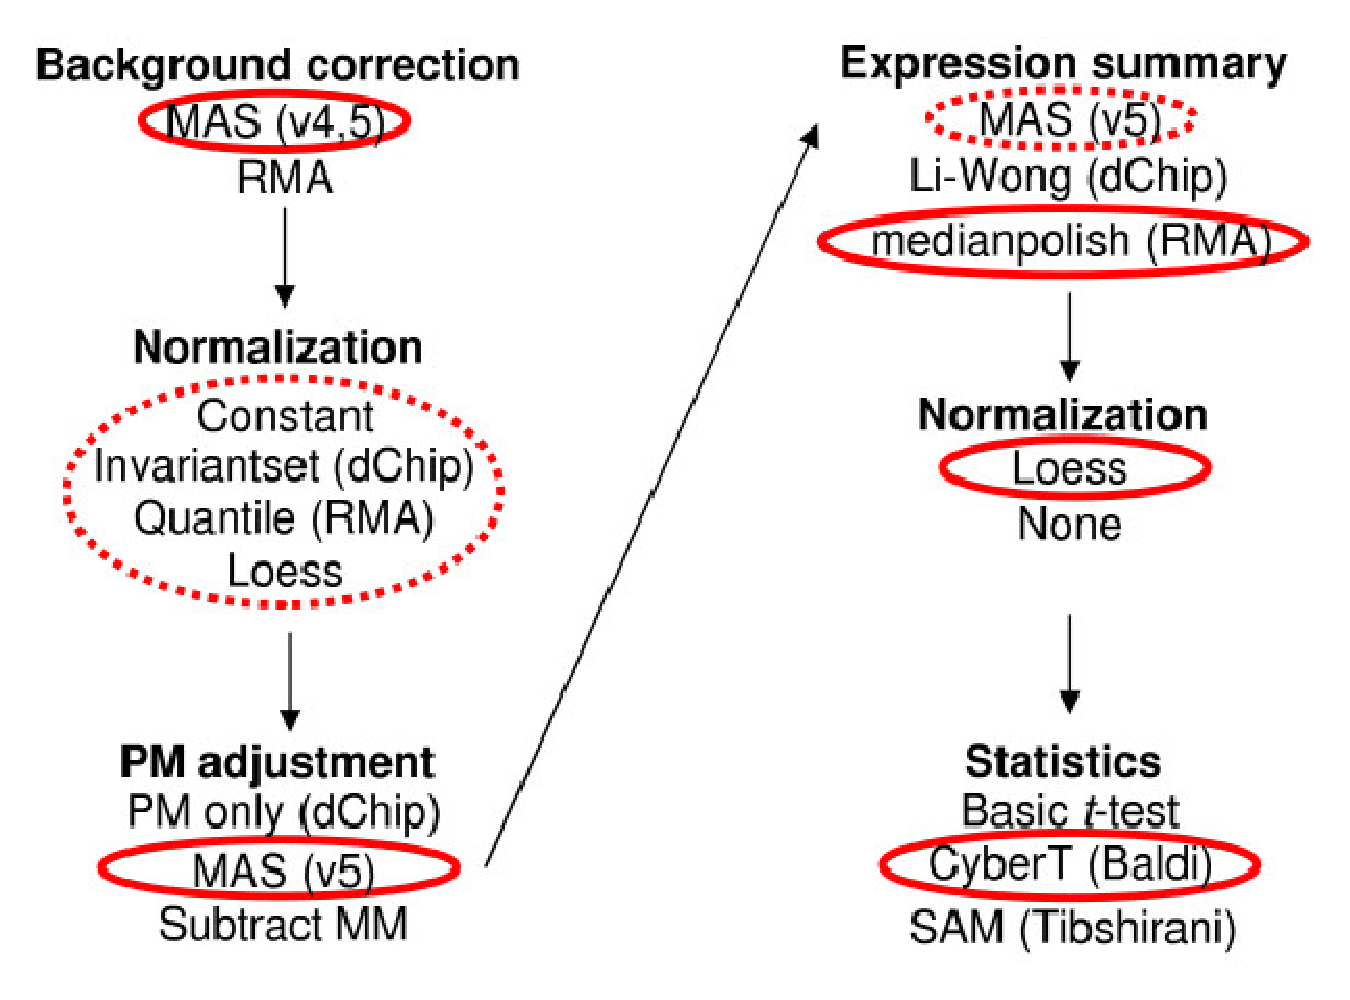
\includegraphics{epsimages/c04preferredAnalysisMethods.eps}}
\end{figure}

Los cap\'itulos que siguen al presente proceden aproximadamente en el orden del proceso descrito en ~\ref{c04preferredAnalysisMethods}.
Se empieza por tratar los principios del dise\~no de experimentos.
A continuaci\'on se describen algunos m\'etodos para el control de calidad, el preprocesado y la normalizaci\'on de los datos.
Se sigue con los m\'etodos de selecci\'on de genes --adaptados de los m\'etodos descritos en el cap\'itulo ~\ref{chapFundEst}, y los m\'etodos de
clasificaci\'on, para concluir con una introducci\'on a los m\'etodos de an\'alisis de la significaci\'on biol\'ogica de las listas de genes obtenidas
de los procesos anteriores.


\chapter{Dise\~no de experimentos de microarrays}

En este cap\'itulo se examinan un componentes clave del an\'alisis de microarrays el dise\~no de experimentos que, no tan s\'olo es
crucial para una buena recogida de informaci\'on sino que marca todo el proceso desde el preprocesado al an\'alisis final.

\section{Fuentes de variabilidad}

Los datos gen\'omicos son muy variables.


\textD{Figura \ref{c04variabilitySources}}{Geschwind (\cite{geschwind:2002} ilustra algunas posibles fuentes de variabilidad, desde que se inicia el experimento hasta que se lee la informaci\'on con el sacnner.}

\vspace{-0.5cm}
\begin{figure}[!h]
\titolfigura[0cm]{Figura \ref{c04variabilitySources}. Proceso de an\'alisis de microarrays}
\label{c04variabilitySources}
\fbox{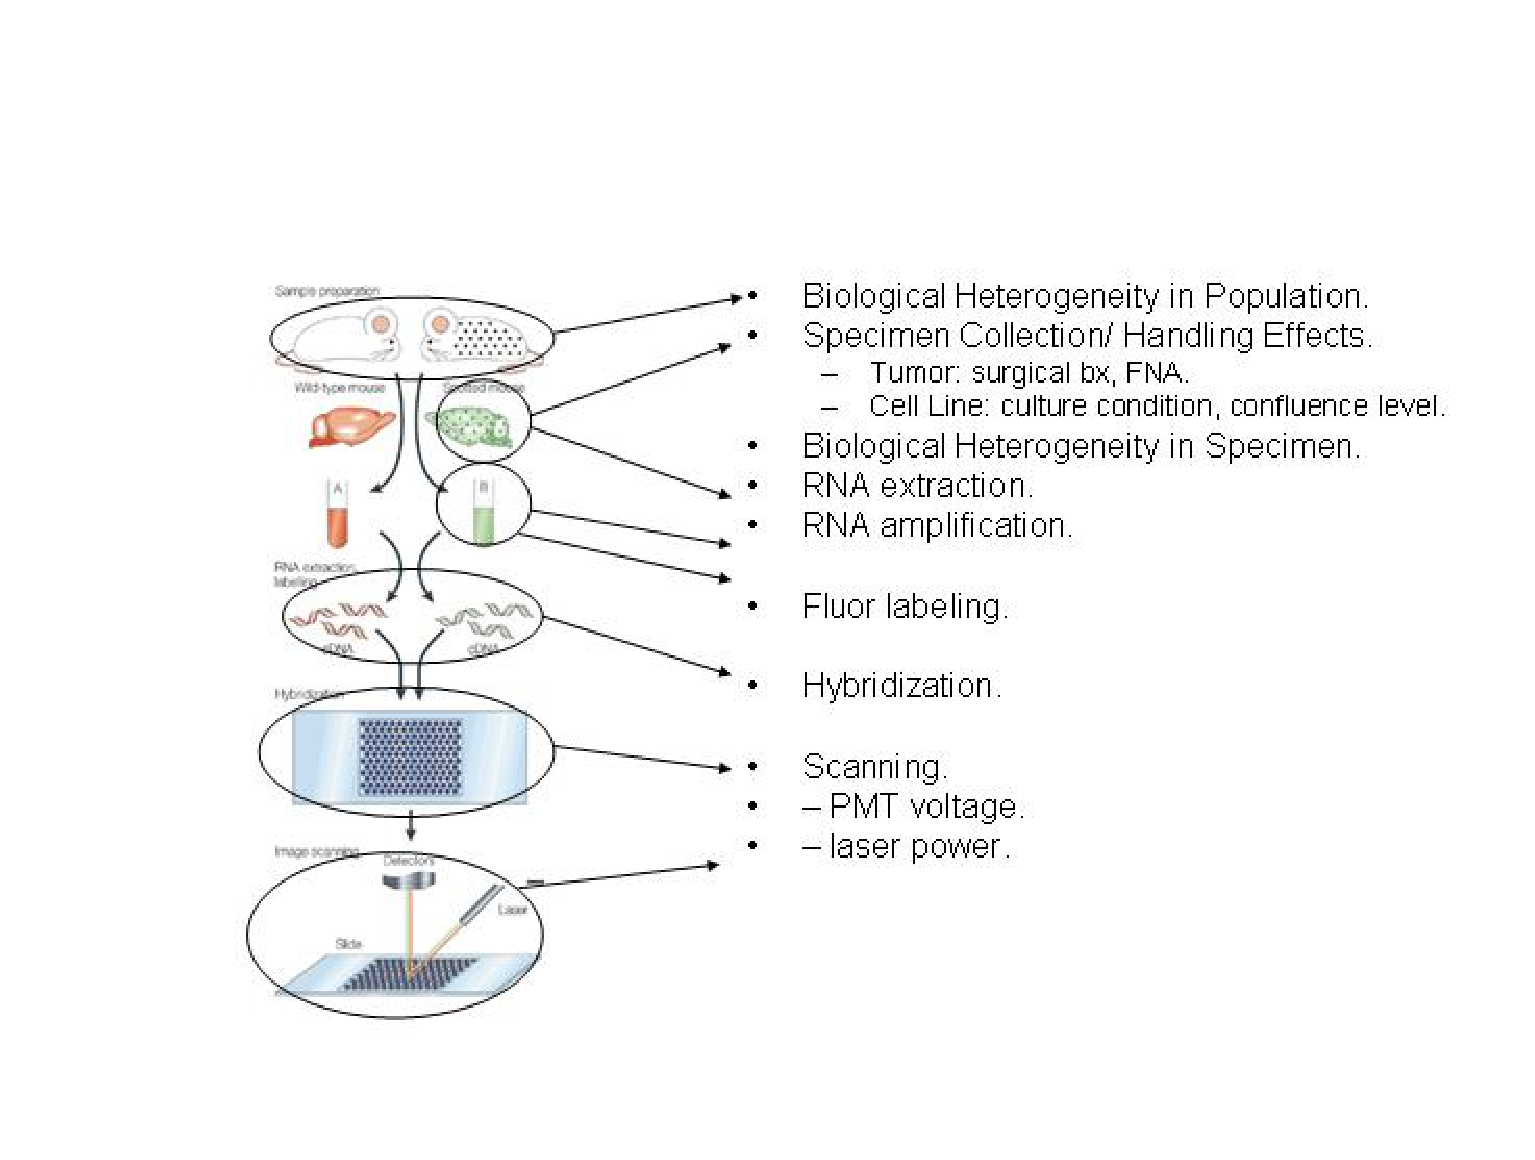
\includegraphics[height=6cm,width=0.75\linewidth]{epsimages/c04variabilitySources.eps}}
\end{figure}


Habitualmente, en la mayor parte de situaciones experimentales, podemos
distinguir entre variabilidad sistem\'atica y aleatoria.

La variabilidad sistem\'atica es principalmente debida a procesos t\'ecnicos
mientras que la variabilidad aleatoria es atribuible tanto a razones t\'ecnicas
como biol\'ogicas. Podemos encontrar ejemplos de variabilidad sistem\'atica en la
extracci\'on del ARN, marcaje o fotodetecci\'on. La variabilidad aleatoria puede
estar relacionada con muchos factores tales como la calidad del ADN o las
caracter\'isticas biol\'ogicas de las muestras.

La manera natural de manejar la variabilidad aleatoria es, por supuesto, la
utilizaci\'on de un dise\~no experimental apropiado y el apoyo para obtener
conclusiones de unas herramientas estad\'isticas adecuadas. Los problemas
relacionados con el dise\~no de los experimentos los discutiremos en esta secci\'on
y los relacionados con la aplicaci\'on de m\'etodos estad\'isticos ser\'an tratados
en la secci\'on  ~\ref{m\'etodos estad\'isticos}.

Tradicionalmente, se estiman las correcciones de la variabilidad sistem\'atica
a partir de los datos, en lo que se llama gen\'ericamente ''calibrado''. En este
contexto, hablaremos de ``normalizaci\'on'', que se tratar\'a en la secci\'on
 ~\ref{preprocesamiento}.

\section{Principales conceptos en Dise\~no de Experimentos}

Vamos a plantear alguna definiciones de conceptos que aparecen de forma usual cuando se plantea un dise\~no:
\begin{itemize}

\item \textbf{Unidad experimental}: Entidad f\'isica a la que se aplica un tratamiento, de forma independiente al resto de unidades. En cada unidad experimental se pueden realizar una medida o varias medidas, en este caso distinguiremos entre unidades experimetales y unidades observacionales. .
\item \textbf{Factor}: son las variables independientes que pueden influir en la variabilidad de la variable de inter\'es.
\item \textbf{Factor tratamiento}: es un factor del que interesa conocer su influencia en la respuesta.
 \item \textbf{Factor bloque}: es un factor en el que no se est\'a interesado en conocer su influencia en la respuesta pero se supone que \'esta existe y se quiere controlar para disminuir la variabilidad residual.
 \item \textbf{Niveles}: cada uno de los resultados de un factor. Seg\'un sean elegidos por el experimentador o elegidos al azar de una amplia poblaci܇n se denominan factores de efectos fijos o factores de efectos  aleatorios.
 \item \textbf{Tratamiento}: es una combinaci\'on espec\'ifica de los niveles de los factores en estudio. Son, por tanto, las condiciones experimentales que se desean comparar en el experimento. En un dise\~no con un \'unico factor son los distintos niveles del factor y en un dise\~no con varios factores son las distintas combinaciones de niveles de los factores.
 \item \textbf{Tama\~no del Experimento}: es el n\'umero total de observaciones recogidas en el dise\~no.
 \end{itemize}

 \section{Principios b\'asicos en el dise\~no del experimento}
 Al planificar un experimento, aparte de la replicaci\'on, hay tres principios b\'asicos que se deben tener siempre en cuenta: 
La replicaci\'on, el control local o ``bloqueo'' y la \textit{aleatorizaci\'on}.
Aplicados correctamente dichos principios garantizan dise\~nos experimentales eficientes.


\section{Replicaci\'on\label{replicacion}}

La replicaci\'on o repetici\'on de un experimento de forma id\'entica en un n\'umero determinado de unidades, es la que
permite la realizaci\'on de un posterior an\'alisis estad\'istico.
La utilizaci\'on de r\'eplicas ss importante para incrementar la precisi\'on, obtener suficiente potencia en los tests y como base para los
procedimientos de inferencia. Normalmente, distinguimos dos tipos de r\'eplicas en el an\'alisis de microarrays:

\begin{itemize}
\item \emph{La replicaci\'on t\'ecnica} se utiliza cuando estamos tratando
r\'eplicas del mismo material biol\'ogico. Puede ser tanto la replicaci\'on
de spots en el mismo chip como la de diferentes alicuotas de la misma muestra
hibridadas en diferentes microarrays.

\item \emph{Replicaci\'on biol\'ogica} se da cuando se toman medidas de m\'ultiples
muestras.

\end{itemize}
La replicaci\'on t\'ecnica permite la estimaci\'on del error a nivel de medida, mientras que
la  replicaci\'on biol\'ogica permite estimar la variabilidad a nivel de poblaci\'on.


\textD{Figura \ref{c04replicas}}{R\'eplicas biol\'ogicas vs t\'ecnicas}

\vspace{-0.5cm}
\begin{figure}[!h]
\titolfigura[0cm]{Figura \ref{c04replicas}.}
\label{c04replicas}
\fbox{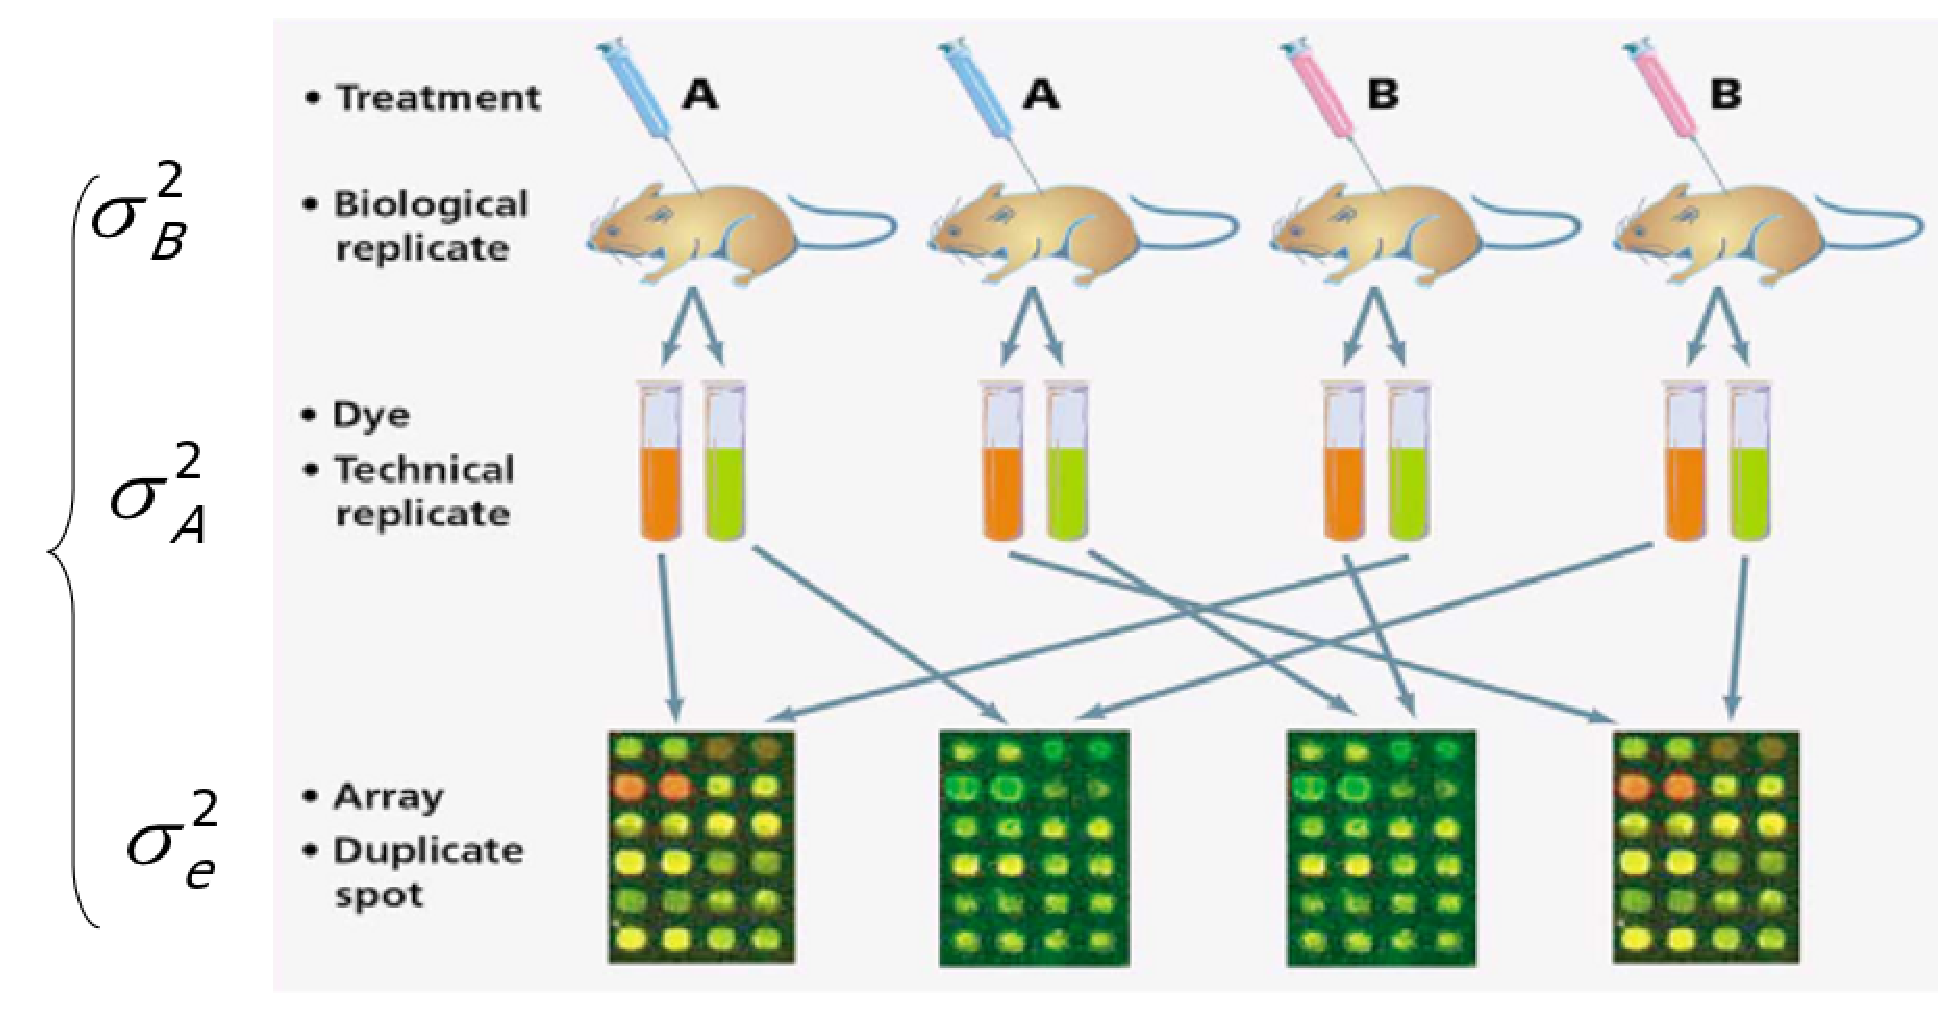
\includegraphics[height=6cm,width=0.75\linewidth]{epsimages/c04replicas.eps}}
\end{figure}


\subsection{Potencia y tama\~no de la muestra\label{samplesize}}

Sorprendentemente, los primeros experimentos de microarrays utilizaban pocas o
ninguna r\'eplica biol\'ogica. La principal explicaci\'on para este hecho - adem\'as
de la falta de conocimiento estad\'istico - fu\'e el alto coste de cada microarray.
En pocos a\~nos, la necesidad de las r\'eplicas ha llegado a ser indiscutible, y al
mismo tiempo, el coste de los chips ha disminuido considerablemente. Actualmente,
es normal la utilizaci\'on de, al menos, tres a cinco r\'eplicas por condici\'on
experimental, aunque a este consenso se ha llegado m\'as por razones emp\'iricas que
por la disponibilidad de modelos apropiados para el an\'alisis de la potencia y
tama\~no de la muestra.

Recientemente, se ha producido una importante afluencia de art\'iculos describiendo
m\'etodos para el an\'alisis de la potencia y tama\~no de la muestra. A pesar de su
variedad, ning\'un m\'etodo aparece como candidato claro para ser utilizado en
situaciones pr\'acticas. Esto se debe, probablemente, a la complejidad de los
datos de microarrays, b\'asicamente por que los genes no son independientes. Por
tanto, estas estructuras de correlaci\'on existen en los datos, pero la mayor parte
de las dependencias son desconocidas por lo que la estimaci\'on de estas estructuras
es muy complicada.

Como indicaba Allison (~\cite{Allison:2006a}) aunque no hay consenso sobre que
procedimiento es mejor para determinar el tama\~no de las muestras, s\'i que lo hay
sobre la conveniencia de realizar el an\'alisis de la potencia, y, por supuesto,
sobre el hecho de que un mayor n\'umero de replicas generalmente proporcionan
una mayor potencia.

\subsection{Pooling\label{pooling}}

En el contexto de los microarrays, llamamos "pooling" a la combinaci\'on de mARN
de diferentes casos en una \'unica muestra. Hay dos razones a favor de ello, una,
es que, a veces, no hay suficiente ARN disponible y esta es la \'unica forma de
conseguir suficiente material para construir los arrays, otra, m\'as controvertida,
es la creencia que la variabilidad entre arrays puede reducirse por "pooling".
La justificaci\'on es que combinar muestras equivale a promediar expresiones, y
como ya se conoce, el promedio es menos variable que los valores individuales. A
pesar de la debilidad de este argumento, es verdad que en ciertas situaciones el
pooling puede ser apropiado y, recientemente, muchos estad\'isticos han dedicado
sus esfuerzos a tratar de responder la pregunta ``to pool or not to pool"
(~\cite{Kerr:2001a}). Por ejemplo, si la variabilidad biol\'ogica est\'a altamente
relacionada con el error en las medidas, y las muestras biol\'ogicas tienen un
coste m\'inimo en comparaci\'on con el de los arrays, una apropiada estrategia de
"pooling" puede ser claramente eficiente en costes.

De todos modos, el "pooling" no se deber\'ia usar en cualquier tipo de estudios.
Si el objetivo es comparar expresiones medias (ver m\'as adelante '' comparaci\'on
de clases''), puede funcionar adecuadamente, pero se deber\'ia claramente evitar
cuando el objetivo del experimento es construir predictores que se basen en
caracter\'isticas individuales.


 \subsubsection{Aleatorizaci\'on}

Se entiende por aleatorizar la asignaci\'on de todos los factores al azar a las unidades experimentales. Co ello se consigue disminuir el efecto de los factores no controlados por el experimentador en el dise\~no experimental y que podr\'ian  influir en los resultados.

Las ventajas de aleatorizar los factores no controlados son:
\begin{itemize}
  \item Transforma la variabilidad sistem\'atica no planificada en variabilidad no planificada o ruido aleatorio. Dicho de otra forma, aleatorizar previene contra la introducci\'on de sesgos en el experimento.
  \item Evita la dependencia entre observaciones al aleatorizar los instantes de recogida muestral.
  \item Valida muchos de los procedimientos estad\'isticos m\'as comunes.
\end{itemize}

\subsubsection{Bloquear}

Hace referencia a dividir o particionar las unidades experimentales en grupos llamados bloques de modo que las observaciones realizadas en cada bloque se realicen bajo condiciones experimentales lo m\'as parecidas posibles.
A diferencia de lo que ocurre con los factores tratamiento, el experimentador no est\'a interesado en investigar las posibles diferencias de la respuesta entre los niveles de los factores bloque.

Bloquear es una buena estrategia siempre y cuando sea posible dividir las unidades experimentales en grupos de unidades similares. La ventaja de bloquear un factor que se supone que tiene una clara influencia en la respuesta pero en el que no se est\'a interesado, es que convierte la variabilidad sistem\'atica no planificada en variabilidad sistem\'atica planificada.


\section{Dise\~nos experimentales para microarrays de dos colores}

En arrays de dos colores, se aplican dos condiciones experimentales a cada array.
Esto permite la estimaci\'on del efecto del array, como el efecto de bloqueo.
En Affymetrix u otro array de un canal, cada condici\'on se aplica a un
chip separado, imposibilitando la estimaci\'on del efecto de los microarrays, lo
cual, por otra parte, se considera que tiene una relaci\'on muy peque\~na en el
tratamiento de los efectos debido al proceso industrial utilizado para fabricar
estos chips.

Como consecuencia de lo anterior, los experimentos que usan arrays de un canal
se consideran ``estandar'', por lo que se les pueden aplicar los conceptos y t\'ecnicas tradicionales de
dise\~no de experimentos .


Los arrays de dos canales presentan una situaci\'on m\'as complicada. Por una parte los
``dos colores'' no son sim\'etricos, es decir, con la misma cantidad de material,
un array hibridado con uno u otro color, sea Cy5 o Cy3, emitir\'a se\~nales con
diferente intensidad. La forma normal de manejar este problema es
 \emph{dye--swapping} que consiste en utilizar para una misma comparaci\'on dos
arrays con dyes cambiados, es decir, si en el primer array la muestra 1 se marca
con Cy3 y la muestra 2 con Cy5, con las muestras del segundo array se hace al
rev\'es (ver figura \ref{c04dyelabels}).


\textD{Figura \ref{c04dyelabels}}{(a) Representaci\'on simplificada de un dise\~no. Cada flecha representa
  un array de dos canales en el que el origen indica el marcaje con Cy3.
  (b) Dye swapping.}

\vspace{-0.5cm}
\begin{figure}[!h]
\titolfigura[0cm]{Figura \ref{c04dyelabels}.}
\label{c04dyelabels}
\fbox{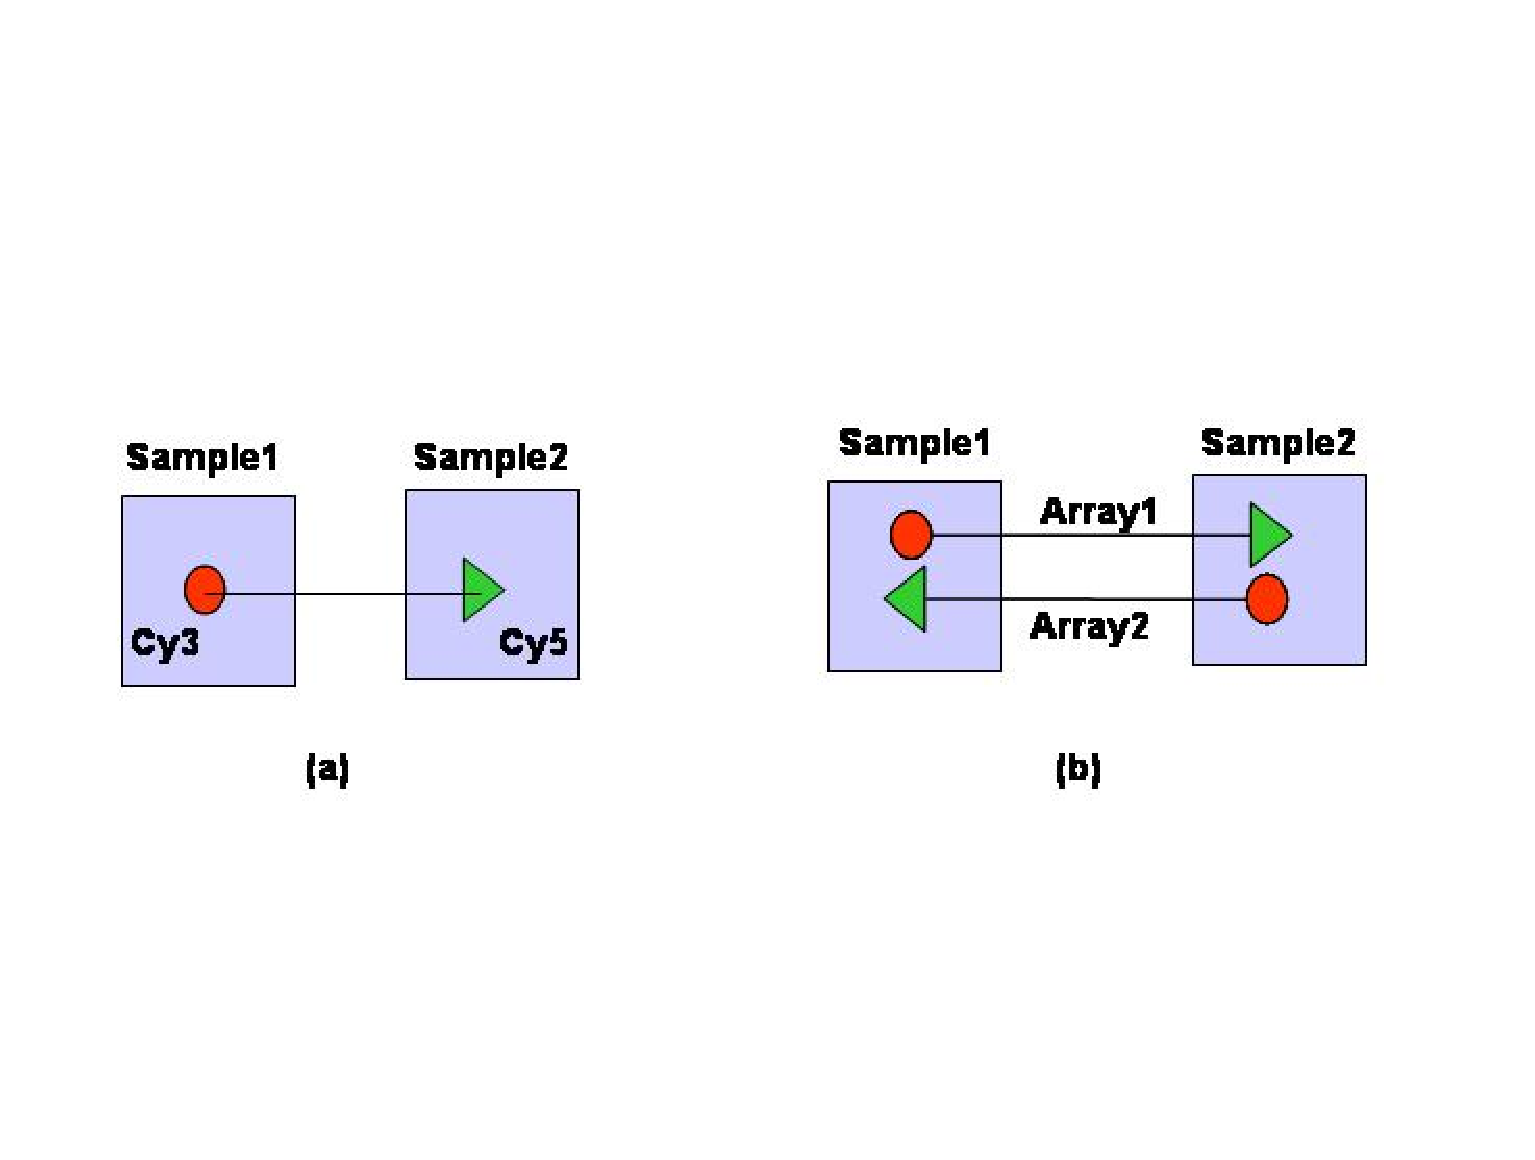
\includegraphics[height=6cm,width=0.75\linewidth]{epsimages/c04dyelabels.eps}}
\end{figure}


Por otra parte, el hecho de que solo se puedan aplicar dos condiciones a cada
array complica el dise\~no, ya sea porque normalmente hay m\'as de dos condiciones,
o porque no es recomendable hibridar directamente dos muestras en un array,
creando pares artificiales.

El problema de la asignaci\'on eficiente de muestras a microarrays, dado un n\'umero
de condiciones a comparar y un n\'umero fijo de arrays disponibles, ha sido
estudiado de forma exhaustiva.

El dise\~no utilizado m\'as comunmente en la comunidad biol\'ogica es el
 \emph{dise\~no de referencia} en el que cada condici\'on de inter\'es se compara
 con muestras tomadas de alguna referencia estandar com\'un a todos las arrays.
(ver figura \ref{c04referencevsloop} (a)).


\textD{Figura \ref{c04referencevsloop}}{(a) Dise\~no de referencia.  (b) Dise\~no en loop.}

\vspace{-0.5cm}
\begin{figure}[!h]
\titolfigura[0cm]{Figura \ref{c04referencevsloop}. Dise\~no de arrays.}
\label{c04referencevsloop}
\fbox{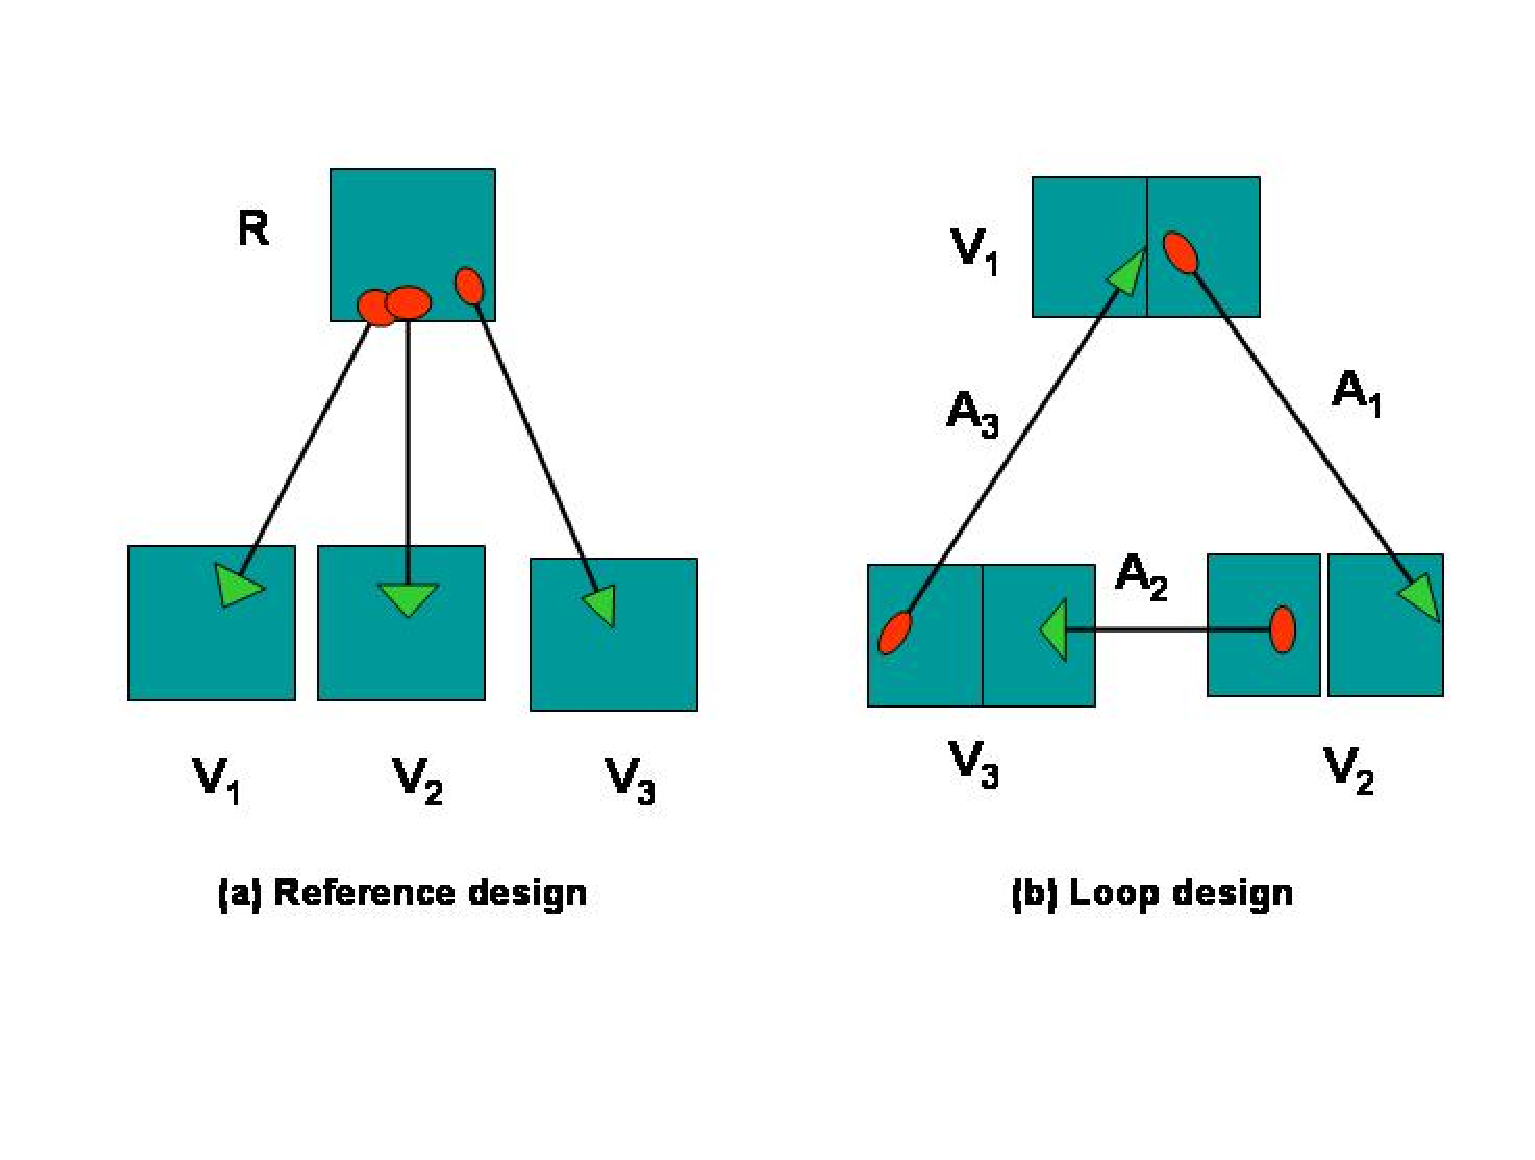
\includegraphics[height=6cm,width=0.75\textwidth]{epsimages/c04referencevsloop.eps}}
\end{figure}

Los dise\~nos de referencia permiten hacer comparaciones indirectas entre
condiciones de inter\'es. La critica m\'as importante a esta aproximaci\'on es que el
50\% de las fuentes de hibridaci\'on se utilizan para  producir la se\~nal del grupo
control, de un inter\'es no intr\'inseco para los bi\'ologos.
En contraste, un dise\~no en loop compara dos condiciones a trav\'es de otra cadena
de condiciones, por lo que elimina la necesidad de una muestra de referencia
 (ver figura \ref{c04referencevsloop}(b)).




\include{capitulo6}
\include{capituloBioconductor}
\include{casoResuelto2}
\include{capitulo7}
\include{casoResuelto3}
%\include{capitulo9}

\newpage
\previs[Resumen]

 El an\'alisis de datos de microarrays \'es una disciplina que combina la bioinform\'atica la estad\'istica y la biolog\'ia para esclarecer problemas que aparecen en el estudio de la expresi\'on g\'enica con microarrays, que son herramientas que permiten el estudio de la expresi\'on de manera simult\'anea en todos los genes de un organismo. Con los microarrays se pueden tratar multitud de problemas entre los que podemos destacar la \emph{comparaci\'on de clases}, el \emph{descubrimiento de nuevos grupos} o la construcci\'on de predictores.


%\newpage
%\epileg{Ejercicios de autoevaluaci\'on}

\%begin{preguntes}
%Pregunta 1
%\item Pregunta 1
%\setcounter{numresp}{0}
%\resposta{Respuesta a}
%\resposta{Respuesta b}
%\resposta{Respuesta c}
%\resposta{Respuesta d}

%Pregunta 2
%\item Pregunta 2
%\setcounter{numresp}{0}
%\resposta{Respuesta a}
%\resposta{Respuesta b}
%\resposta{Respuesta c}
%\resposta{Respuesta d}

%Pregunta 3
%\item Pregunta ...
%\setcounter{numresp}{0}
%\resposta{Respuesta a}
%\resposta{Respuesta b}
%\resposta{Respuesta c}
%\resposta{Respuesta d}
%\end{preguntes}

%\newpage
%\epileg{Solucionario}

%\small
%\setlength{\parskip}{10pt}

%\textsbold{1.} d; \textsbold{2.} d; \textsbold{3.} a; ...


%\epileg{Glosario}

%\textbf{Palabra 1} Definici\'on

%\textbf{Palabra 2} Definici\'on

%\textbf{Palabra 3} Definici\'on

%\bibliografia


\bibliographystyle{plain}

\bibliography{MDAreview}





\end{document}


%%% Local Variables: 
%%% mode: latex
%%% TeX-master: t
%%% End: 
